\documentclass[12pt,a4paper]{scrartcl}

\usepackage[a4paper, left=2cm, right=1cm, bottom=1cm, top=1cm, includeheadfoot]{geometry}
\usepackage[ngerman]{babel}
\usepackage[utf8]{inputenc} % comment this if you uncomment utf8x
%\usepackage[utf8x]{inputenc} % uncomment this if there are problems with 'ä', 'ü', 'ö'
\usepackage{ucs}
\usepackage[usenames,dvipsnames]{xcolor}
\usepackage[fleqn]{amsmath}
\usepackage{amsfonts}
\usepackage{amssymb}
\usepackage{color}
\usepackage{listings}
\usepackage{hyperref}
\usepackage{amsfonts}
\usepackage{listings}
\usepackage{scrpage2}
\usepackage{graphicx}


\definecolor{mygray}{rgb}{0.9,0.9,0.9}
\lstset{language=[Visual]Basic, morekeywords={param, local}}


\lstset{
   literate={ö}{{\"o}}1
           {ä}{{\"a}}1
           {ü}{{\"u}}1
           {ß}{{\ss}}1
           {é}{{\'e}}1,
   inputencoding=ansinew,
   extendedchars=true,
   basicstyle=\scriptsize\ttfamily,
   numberstyle=\scriptsize,
   breaklines=true,
   tabsize=2,
   numbersep=5pt
}
\lstdefinestyle{customcpp}{
   language=C++,
   backgroundcolor=\color{mygray},
   numbers=left,
   keywordstyle=\color{blue}\bfseries,
   stringstyle=\color{BrickRed}\ttfamily,
   commentstyle=\color{OliveGreen}\ttfamily,
   showspaces=false,
   showstringspaces=false,
   showtabs=false
}
\lstdefinestyle{customoutput}{
   backgroundcolor=\color{mygray},
   numbers=none,
   showspaces=false,
   showtabs=false
}

\newcommand{\sourceCode}[1]{\lstinputlisting[style=customcpp]{#1}} %beinhaltet alle benötigten Packages etc.
\begin{document}
\graphicspath{{./}}

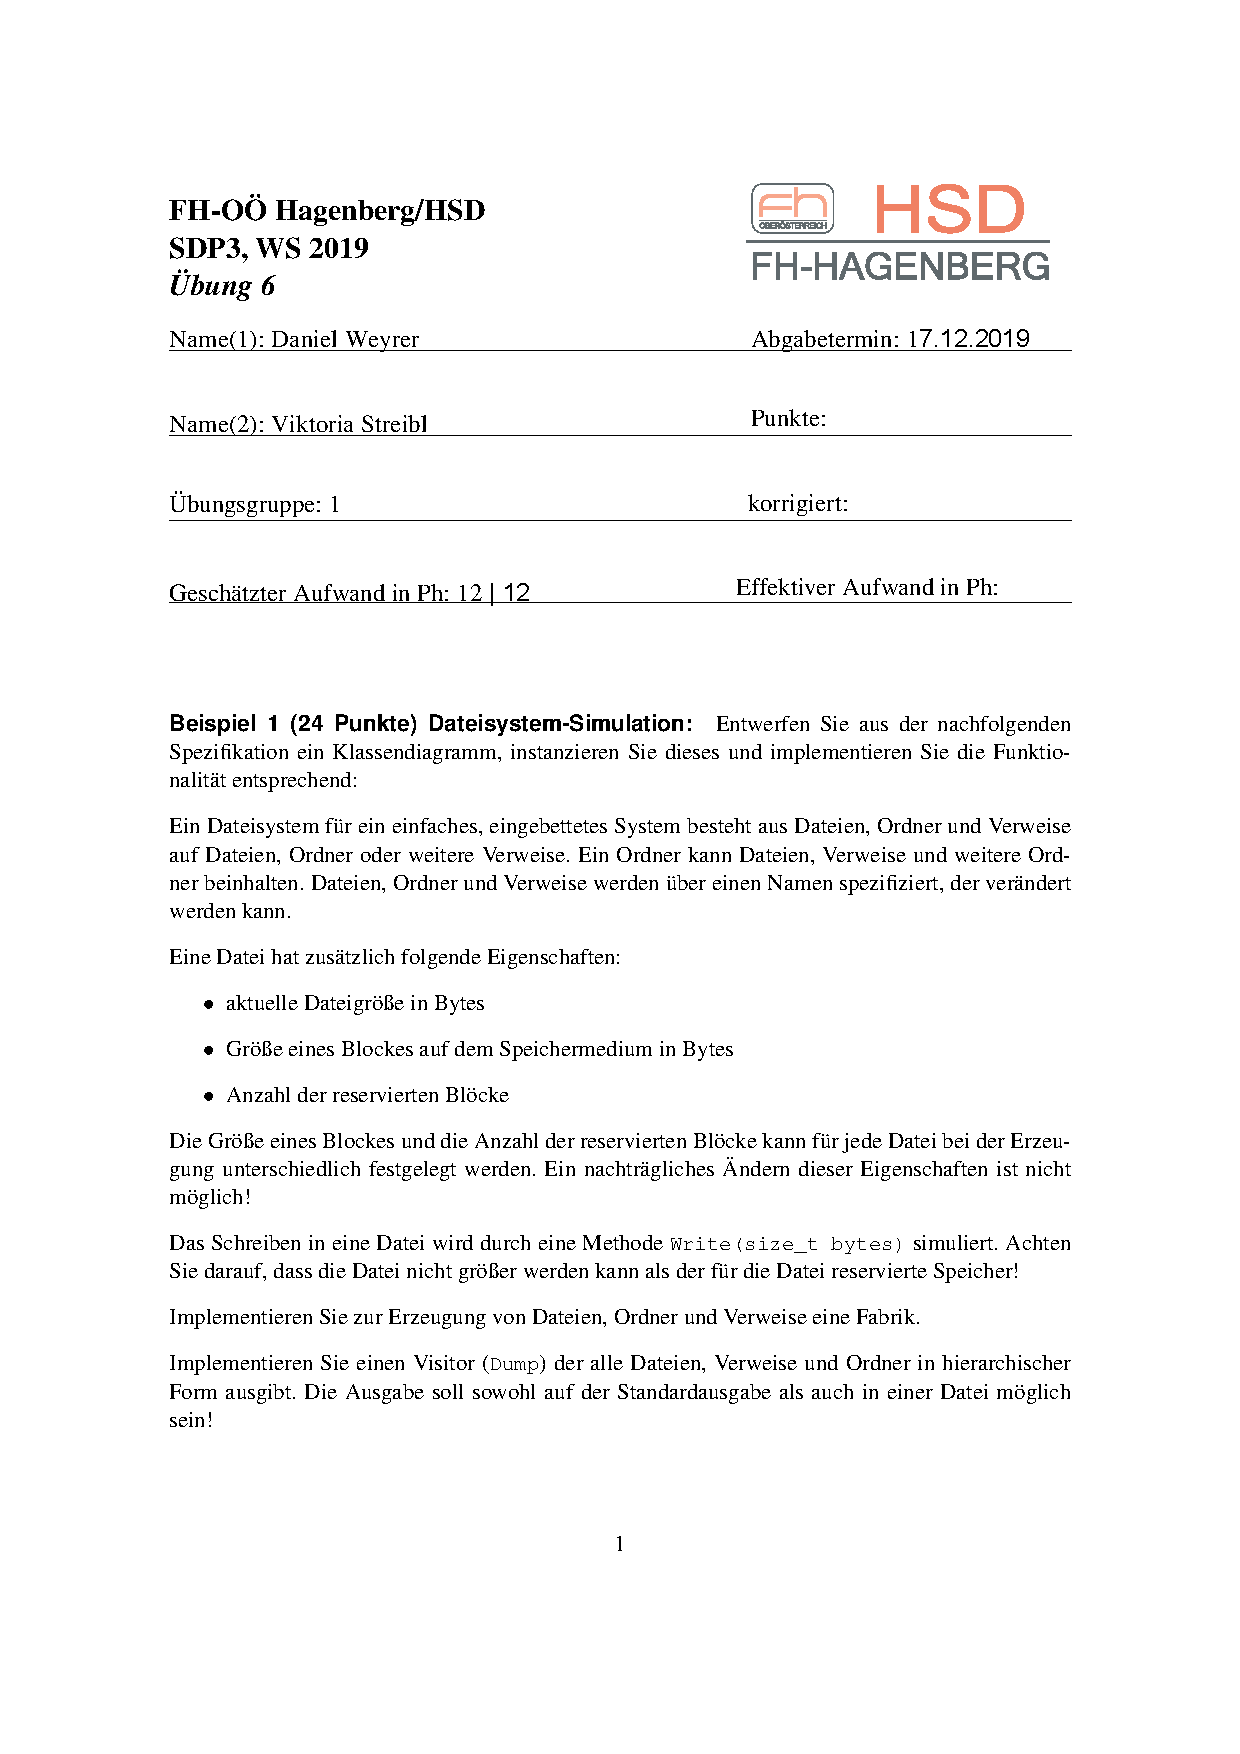
\includepdf[pages=-]{../Angabe.pdf}

\title{SDP - Exercise 06} % Übungsname und Nummer angeben
\subtitle{winter semester 2019/20} % Semester angeben oder auskommentieren, falls nicht erwünscht
\author{
Viktoria Streibl - S1810306013\\
  Daniel Weyrer - S1820306044
} % Autorenname
\date{\today} % Das heutige Datum automatisch einfügen

\maketitle % Titelseite erstellen

\newpage
\tableofcontents % Inhaltsverzeichnis erstellen
\newpage

\ihead{Viktoria Streibl}
\ohead{Daniel Weyrer}
\chead{SDP3-UE Uebung 06}

\section{Organizational}
\subsection{Team}
\begin{itemize}
	\item Viktoria 	Streibl 		- 	S1810306013
	\item Daniel 	Weyrer		-	S1820306044
\end{itemize}

\subsection{Roles and responsibilities}
\subsubsection{Jointly}
\begin{itemize}
	\item Planning
	\item Documentation
	\item Systemdocumentation
	\item Class Diagram
	\item Class FileSystem
	\item TestDriver
\end{itemize}

\subsubsection{Viktoria Streibl}
\begin{itemize}
	\item Visitors
	\subitem Visitor Dump
	\subitem Visitor FilterFiles			
\end{itemize}

\subsubsection{Daniel Weyrer}
\begin{itemize}
	\item Base Class Type
	\item Derived Classes
		\subitem Class File
		\subitem Class Referral
		\subitem Class Folder
	\item Factory
\end{itemize}

\subsection{Effort}

\subsubsection {Viktoria Streibl}
\begin{itemize}
	\item estimated: 12 ph 
	\item actually: 6 ph
\end{itemize}

\subsubsection {Daniel Weyrer}
\begin{itemize}
	\item estimated: 12 ph 
	\item actually: 10 ph
\end{itemize}

\section{Requirenment Definition(System Specification)}
The Filesystem should work like a Linux-Based Filesystem. It can contain Files, Folders and Referrals. The Referrals can refer to a File or a Folder.

\section{System Design}
\newpage
\subsection{Classdiagram}
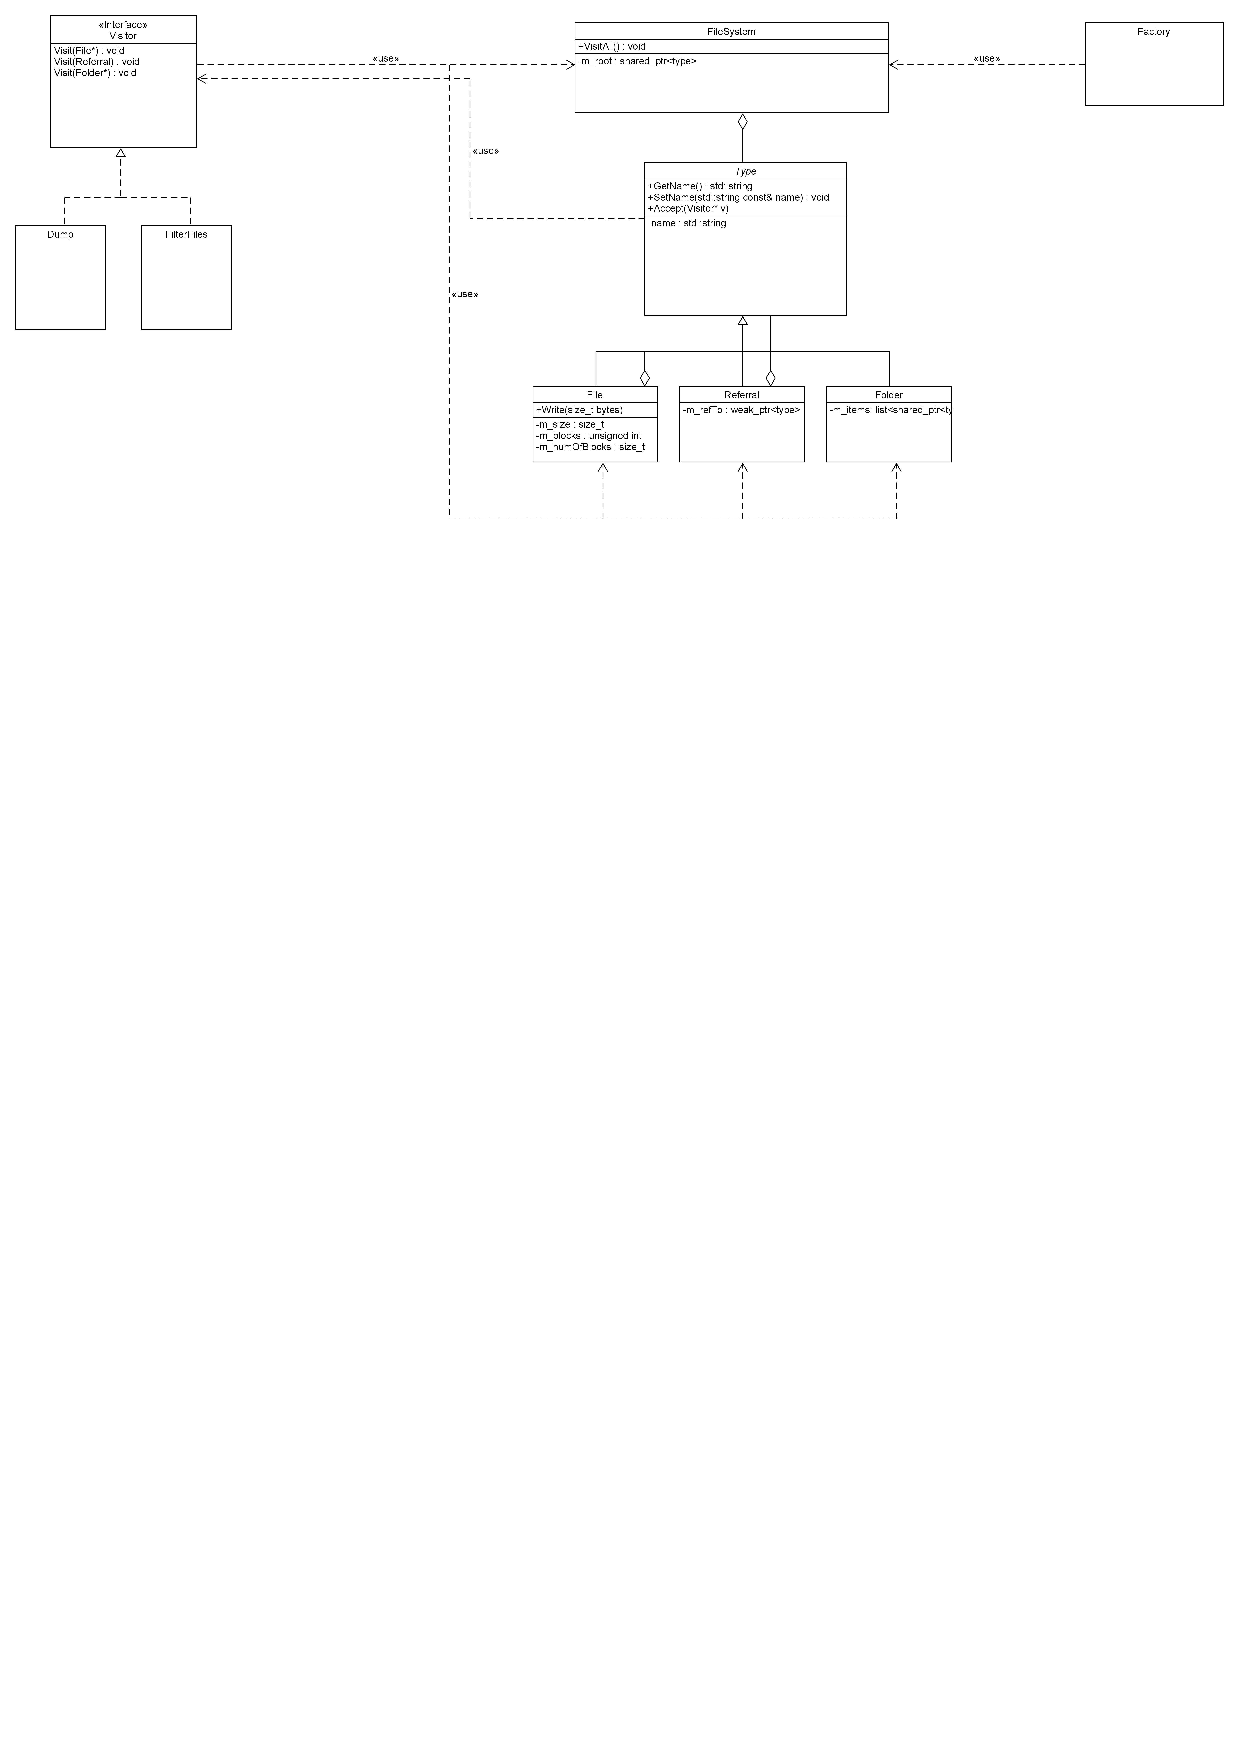
\includegraphics[scale=1, angle=90]{../ClassDiagram.pdf}

\subsection{Design Decisions}
\subsubsection{Using a Folder as Root}
As we wanted to make a Filesystem comparable to the Linux-FS, we chose a Folder as the root of the whole System! 

\subsubsection{Empty Implementations}
As we used pointers of type "Type" we had to make some Functions pure virtual to call them by the pointer. As a File has no list of pointers as Member, we had to keep the Methods empty

\subsubsection{Add-Function}
We chose to Add Objects by using a path (std::string) as location-giving variable, which comes as close as possible to a "real" linux-filesystem


\section{Component Design}
\subsection{Filesystem}
This class is the for the company Epos and uses the interface IEpos.
\begin{itemize}
\item void EncryptRSA(fileName)
\subitem It calls the method EncryptRSA of the interface.
\item void DecryptRSA(fileName)
\subitem It calls the method DecryptRSA of the interface.
\end{itemize}

\subsection{Client Nortel Networks}
This class is the for the company Epos and uses the interface INortelNetworks, it contains following functions:
\begin{itemize}
\item void Encipher(type, fileName)
\subitem It calls the method Encipher of the interface.
\item void Decipher(type, fileName)
\subitem It calls the method Decipher of the interface.
\end{itemize}

\subsection{Interface IEpos}
This interface holds the following functions:
\begin{itemize}
\item virtual  void EncryptRSA(fileName)
\subitem Defines a function for encrypting a file via RSA.
\item virtual void DecryptRSA(fileName)
\subitem Defines a function for decrypting a file via RSA.
\end{itemize}

\subsection{Interface INortelNetworks}
This interface holds the following functions:
\begin{itemize}
\item virtual  void Encipher(type, fileName)
\subitem Defines a function for encrypting a file with the algorithm of the specific type.
\item virtual void Decipher(type, fileName)
\subitem Defines a function for decrypting a file with the algorithm of the specific type.
\end{itemize}

\subsection{Adaptor AEpos}
This class is an adapter for the Interface IEpos. It contains following methods:
\begin{itemize}
\item void EncryptRSA(fileName)
\subitem Implements the function of the Interface. It calls the RSA encrypting algorithmn and encrypts the file.
\item void DecryptRSA(fileName)
\subitem Implements the function of the Interface. It calls the RSA decrypting algorithmn and decrypts the file.
\end{itemize}

\subsection{ANortelNetworks}
This class is an adapter for the Interface INortelNetworks. It contains following methods:
\begin{itemize}
\item void Encipher(type, fileName)
\subitem Implements the function of the Interface. It checks which kind of encoding type it should use and calls
the respective algorithmn of encrypting.
\item void Decipher(type, fileName)
\subitem Implements the function of the Interface. It checks which kind of encoding type it should use and calls
the respective algorithmn of decrypting.
\end{itemize}

\subsection{Class Encryptor}
Base Class, contains base-functionality such as:
\begin{itemize}
\item void GenFile(fileName, content)
\subitem Creates new File with the given Filename and writes the content into the file

\item string ReadFile(fileName)
\subitem Reads of the file with the given File-name into a string and returns the string.

\item string NewFileEnding(oldFileName, oldFileEnding, newFileEnding (, appendix)
\subitem Checks for correct file-ending of the file and creates a new one with the new file-extension and optional with an appendix (to create "filename decrypted.txt"). Throws an exception if the file has the wrong file-extension, returns string with new Filename (and extension) otherwise.
\end{itemize}

\subsection{Class Caesar}
Derived class, responsible for the Caesar-Encryption
\begin{itemize}
	\item Caesar()
	\subitem Sets default encryption-key
	
	\item Encrypt(fileName)
	\subitem Main Encryptionfunction, responsible for the whole encryption process:
	\subsubitem Check file for correct ending
	\subsubitem Read file to a String
	\subsubitem create a encrypted string (character by character)
	\subsubitem create a file with the new file extension ".caesar" 
	\subsubitem Write encrypted string to the newly created file
	
	\item Decrypt(fileName)
	\subitem Main Decryptionfunction, responsible for the whole decryption process:
	\subsubitem Check for correct file extension
	\subsubitem Read File to a string
	\subsubitem create a decrypted string
	\subsubitem create a new file with "-decrypted.txt" ending and extension
	\subsubitem write the decrypted string to the newly created file
\end{itemize}
\subsection{Class RSA}
Derived class, responsible for the RSA-Encryption
\begin{itemize}
	\item Caesar()
	\subitem Sets default encryption-keys
	
	\item Encrypt(fileName)
	\subitem Main Encryptionfunction, responsible for the whole encryption process:
	\subsubitem Check file for correct ending
	\subsubitem Read file to a String
	\subsubitem create a encrypted string (character by character)
	\subsubitem create a file with the new file extension ".RSA" 
	\subsubitem Write encrypted string to the newly created file
	
	\item Decrypt(fileName)
	\subitem Main Decryptionfunction, responsible for the whole decryption process:
	\subsubitem Check for correct file extension
	\subsubitem Read File to a string
	\subsubitem create a decrypted string
	\subsubitem create a new file with "-decrypted.txt" ending and extension
	\subsubitem write the decrypted string to the newly created file
	
	\item CalcPowMod(c, pow, mod)
	\subitem Based on the RSA Algorithm, it is needed to calculate \(c^{pow} \bmod mod\). This function splits the calculation into pieces to avoid high numbers.
\end{itemize}

\subsection{TestDriver}
The Testdriver test alle functions of the clients. It tests the interface for the Epos-Company as well as the NortelNetwork-Company. It encrypt and decrypt several files. It contains also some functions:
\begin{itemize}
\item int main()
\subitem It calls all tests.

\item void CreateFullTest(subtitle, filename)
\subitem This function calls the function to print the title of the tests. Then i tests the Epos functionality and the Nortel Network functionality.

\item void testEPOS(fileName)
\subitem It calls at first the encrypting method of the specific file and than the decrypting method.

\item void testNN(type, fileName)
\subitem It calls at first the encrypting method of the specific file tests all encoding types, than it decrypts the outcome.

\item void PrintSubheader(subtitle)
\subitem This function outputs the title of the following test.
\end{itemize}
Following tests are implemented:
\begin{itemize}
\item Test alphabet and numbers
\item Test special characters
\item Testing an email file
\item Test if no file is there
\item Test if file is empty
\end{itemize}
It ouputs a error message if there was no successful run.

\newpage
\section{Test Protocol}

\subsection{Testfiles}
\subsubsection{}

\newpage
\section{Source Code}

\subsection{FileSystem}
\subsubsection{FileSystem.h}
\sourceCode{../../FileSystem/FileSystem/FileSystem.h}
\subsubsection{FileSystem.cpp}
\sourceCode{../../FileSystem/FileSystem/FileSystem.cpp}
\newpage

\subsection{Type}
\subsubsection{Type.h}
\sourceCode{../../FileSystem/FileSystem/Type.h}
\subsubsection{Type.cpp}
\sourceCode{../../FileSystem/FileSystem/Type.cpp}
\newpage

\subsection{File}
\subsubsection{File.h}
\sourceCode{../../FileSystem/FileSystem/File.h}
\subsubsection{File.cpp}
\sourceCode{../../FileSystem/FileSystem/File.cpp}
\newpage

\subsection{Referral}
\subsubsection{Referral.h}
\sourceCode{../../FileSystem/FileSystem/Referral.h}
\subsubsection{Referral.cpp}
\sourceCode{../../FileSystem/FileSystem/Referral.cpp}
\newpage

\subsection{Folder}
\subsubsection{Folder.h}
\sourceCode{../../FileSystem/FileSystem/Folder.h}
\subsubsection{Folder.cpp}
\sourceCode{../../FileSystem/FileSystem/Folder.cpp}
\newpage

\subsection{IVisitor}
\subsubsection{IVisitor.h}
\sourceCode{../../FileSystem/FileSystem/IVisitor.h}
\subsubsection{IVisitor.cpp}
\sourceCode{../../FileSystem/FileSystem/IVisitor.cpp}
\newpage

\subsection{Dump}
\subsubsection{Dump.h}
\sourceCode{../../FileSystem/FileSystem/Dump.h}
\subsubsection{Dump.cpp}
\sourceCode{../../FileSystem/FileSystem/File.cpp}
\newpage

\subsection{FilterFiles}
\subsubsection{FilterFiles.h}
\sourceCode{../../FileSystem/FileSystem/FilterFiles.h}
\subsubsection{FilterFiles.cpp}
\sourceCode{../../FileSystem/FileSystem/FilterFiles.cpp}
\newpage

\subsection{Factory}
\subsubsection{Factory.h}
\sourceCode{../../FileSystem/FileSystem/Factory.h}
\subsubsection{Factory.cpp}
\sourceCode{../../FileSystem/FileSystem/Factory.cpp}
\newpage

\subsection{TestDriver}
\subsubsection{TestDriver.cpp}
\sourceCode{../../FileSystem/FileSystem/TestDriver.cpp}
\newpage




\end{document}